\subsection{Perceptron} \label{subs:perceptron}
The perceptron was first developed in 1957 by \textcite{brain_perceptron_nodate}. It is a computational model based on on the brain. The human brain has a huge number of computing units, \textbf{neurons}. A biological neuron receives information (collects charges) from synapses through chemical mechanisms and once a threshold is passed, the cumulate charges are released (we say the neuro fires) and the information is transmitted to other neurons.

Mathematically, a perceptron has n inputs ($x_1$, ..., $x_n$) which can be expressed as vector \textbf{$\bar{x}$}, n wheights (\textbf{$\bar{w}$}) and a bias \textbf{b}. The perceptron, when receiving an input vector, performs a weighted sum. If the wheighted sum is above a threshold (controlled by the bias which can lower or raise it), the perceptron is 'activated' and outputs a non-zero value (1). The figure \ref{fig:perceptron} illustrates this. We can write the operation in a vector form:
%
$$
h(x| w, b) = h(\sum^{n}_{i=1} x_i \cdot w_i + b) = h ( \textbf{$\bar{w}$}^{T} \textbf{$\bar{x}$} + b)
$$
%
where $h$ is the activation function of the perceptron (the section \ref{subs:acti} describes other activation functions)
$$
h ( \textbf{$\bar{w}$}^{T} \textbf{$\bar{x}$} + b) = \begin{cases} 1, & \mbox{if } \textbf{$\bar{w}$}^{T} \textbf{$\bar{x}$} + b > 0 \\ 0, & \mbox{Otherwise} \end{cases}
$$
In the following section \ref{subs:fcl}, we discover how we can use mutliple perceptrons to create a \textbf{fully-connected layer}.
%
\begin{figure}
    \centering
    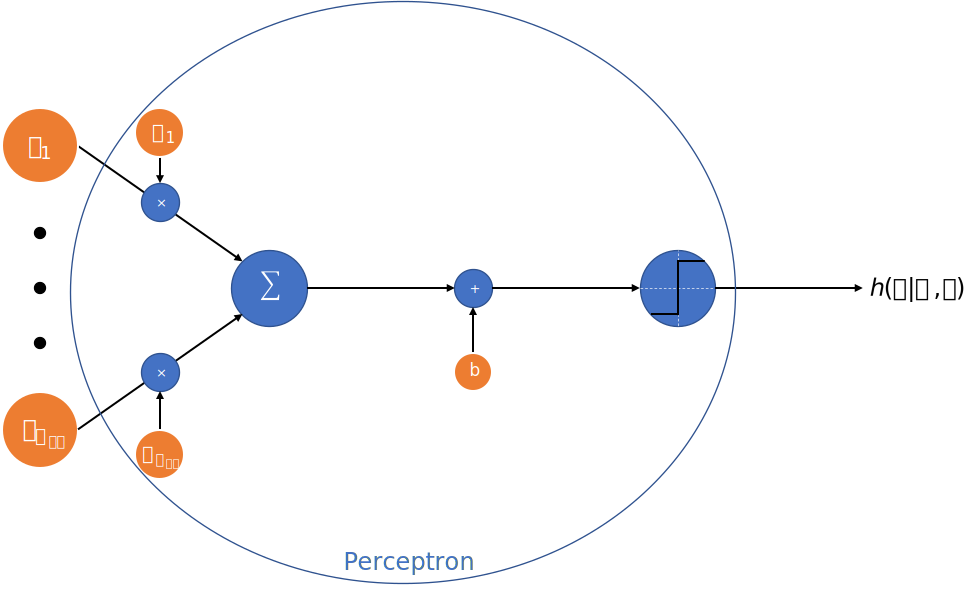
\includegraphics[width=\textwidth]{perceptron.pdf}
    \caption{The Perceptron}
    \label{fig:perceptron}
\end{figure}
